\documentclass[main.tex]{subfiles}

\begin{document}
	
	\begingroup
	
	\renewcommand{\cleardoublepage}{}
	
	\renewcommand{\clearpage}{}
	
	\chapter{Storing Groceries Task Overview}
	
	\chapterauthor{Torge Olliges, Tom-Eric Lehmkuhl, Evan Kapitzke, Jeremias Thun}

	\section{Goal}
	The goal of the Storing Groceries task is, like the name indicates, to store several groceries at their designated position. For the RoboCup this task has been simplified. The objects are all on a table and need to be sorted into a predefined shelf. The sorting has to be done by categories which need to be comprehensible by a human. This can be based on color, form or other categories. To fulfill this task the HSR has to identify the objects on the table and existing objects in the shelf. Furthermore it needs to grasp and place one object after the other. It also needs to navigate between the shelf and table. For additional points the HSR has to open doors. Overall the HSR has only 5 minutes to complete the task. 

	\section{Tasks}
	The figures \ref{grocery_seq_01} and \ref{grocery_seq_02} show the procedure of Storing Groceries. The following subsections explain the execution and procedure in detail and give insights into the decisions made resulting in the exact plan depicted below. Additionally a more in depth explanation of some of the challenges will be given.
	
		\begin{figure}[H]
			\centering
			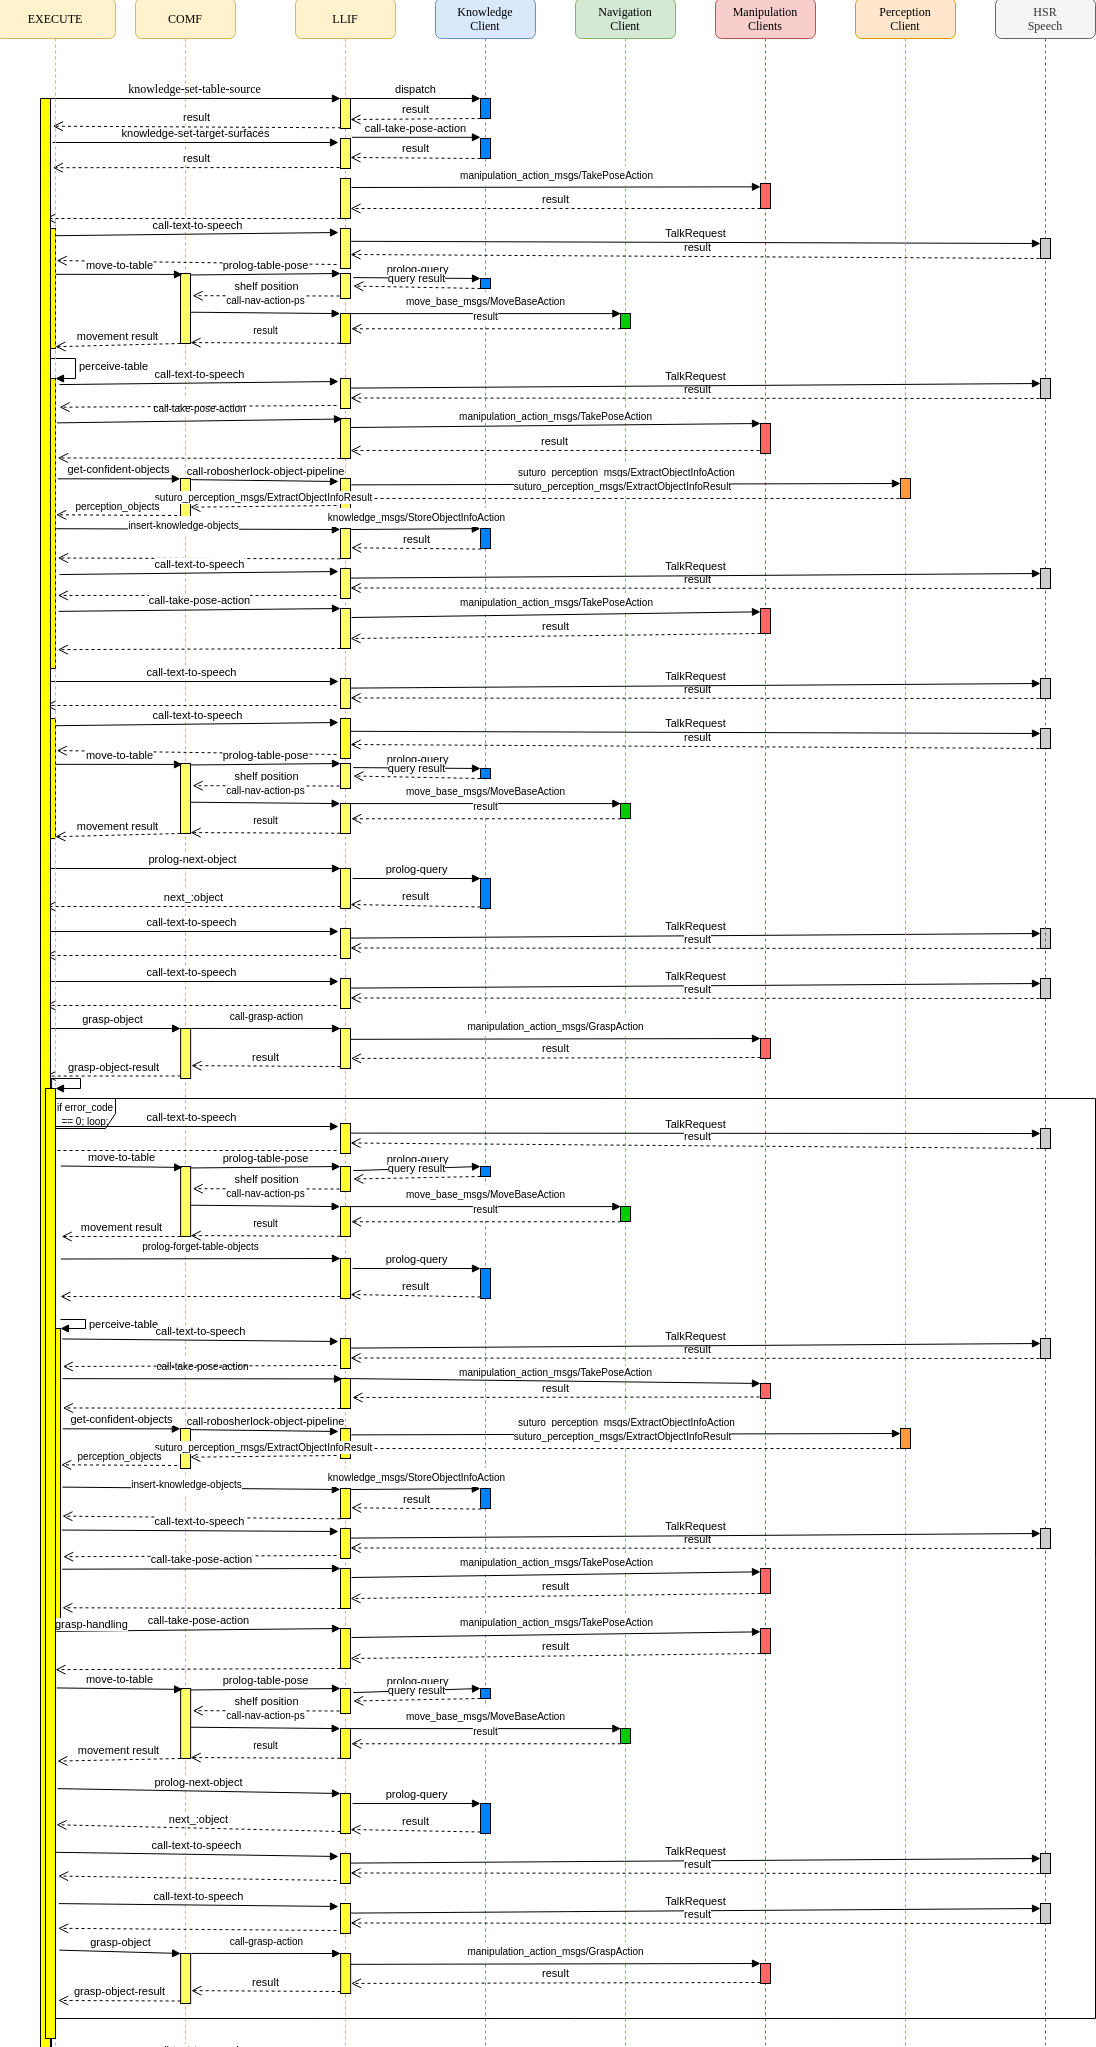
\includegraphics[width=0.85\textwidth]{pictures/diagramms/first-part-grocery-sequence.png}
			\caption{Sequence diagram of the complete run of the grocery storing task \textit{(explanations below)}}
			\label{grocery_seq_01}
		\end{figure}
		\begin{figure}[H]
			\centering
			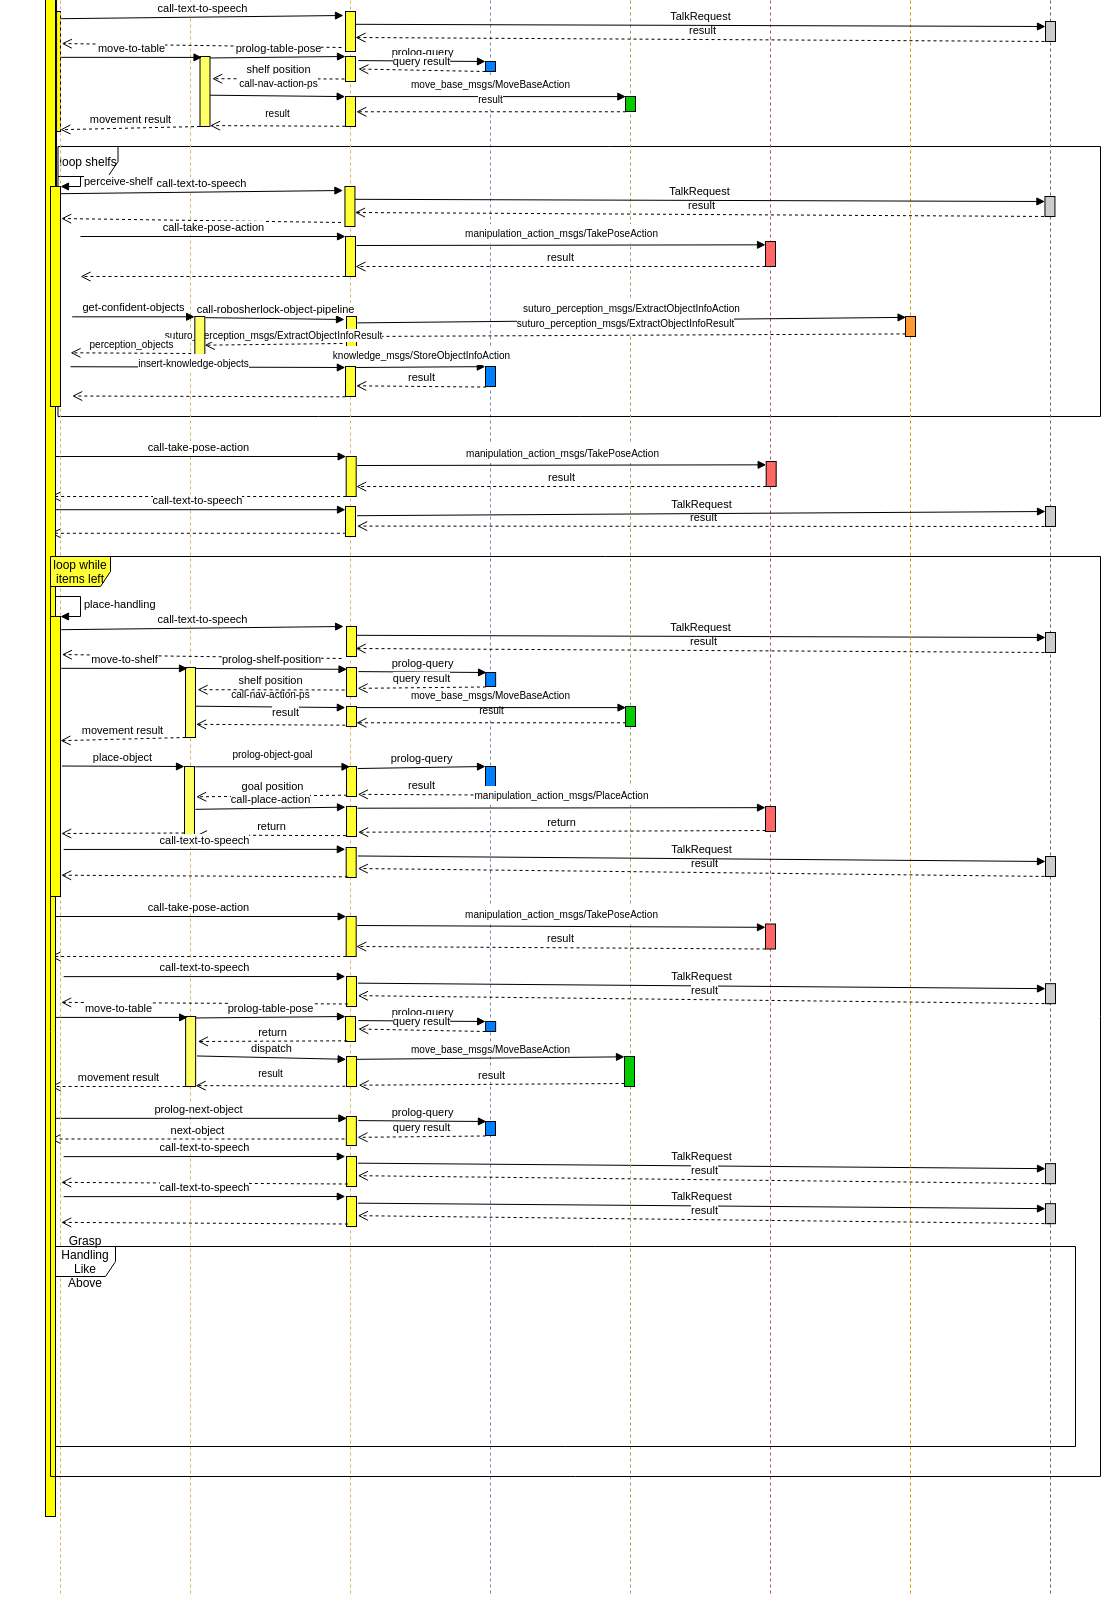
\includegraphics[width=0.85\textwidth]{pictures/diagramms/second-part-grocery-sequence.png}
			\caption{Sequence diagram of the complete run of the grocery storing task \textit{(explanations below)}}
			\label{grocery_seq_02}
		\end{figure}
		\textit{The sequence diagram in figure \ref{grocery_seq_01} and \ref{grocery_seq_01} does not depict when the action servers are running it rather displays the time they are actively used.}
	
	\subsection{Setup}
	

	% Knowledge: set-tables-source 
	According to the task only one table serves as the \texttt{source} for objects. In Knowledge it is allowed to set multiple \texttt{sources} for objects in order to allow greater compatibility and easier adaption to other tasks. For the current task at hand only the corresponding table is set as \texttt{source}. The same principle applies to the shelf which is set as \texttt{target} surface. Every surface e.g. tables, shelf's or the floor can be set as \texttt{source} or \texttt{target}.
	
	\subsection{Scan Table}
	
	% Manipulation: take pose action
	The robot is set to the default pose to make sure it is in a neutral state. This is important in order to avoid moving the robot for example with an extended arm. Manipulation allows the use of predefined poses as well as setting a pose by defining the joint states. These joint states are the forwarded to Giskard.
	
	% NLP: Talk Request
	
	The talk requests are used to inform the developer as well as the people following the robot or evaluating its behavior about what the robot is about to do. They are also used for safety measures so the robot can warn when it is going to move so bystanders can step aside. 
	
	% Knowledge: get table-poses
	Knowledge finds all the tables available, sorts them by their distance to the robot and then returns the list of their position to Planning, so that Planning can determine where to go next.
	
	% Navigation: moveBaseAction
	Planning determines a goal for the move base action. In this goal the HSR is turned $90^\circ$ to the table. Allowing it to look over its shoulder having a clear view of the table without the arm in its way. The default navigation client of the HSR then executes the action. 
	
	% NLP
	Informing that the robot is perceiving the table now.
	
	% Manipuilation: TakePoseAction
	Manipulation gets the task to put the HSR into a pose to perceive an object depending on the height of the plane the object is on.
    That is necessary for Perception to get a good angle and distance to the object and to avoid having the robots arm block the cameras view.
	
	% Perception: Percieve and return data
	The HSR takes a picture of the scene it is currently looking at and processes it with RoboSherlock. Based on the requested region the input images are filtered. The results are then published by the \textit{perception\_actionserver}.
	
	% Knowledge: Store Data
	Knowledge checks the data of the object, that is supposed to be stored. If the class is unknown to Knowledge, it is set to other. If the data is valid the object gets added to the knowledge base and the objects at the position of the new object are put into a group.
	% NLP: Talk Request
	
	% Manipulation: Take pose
	In order to grasp a object the HSR needs to look straight at the object with its base. Therefore the HSR needs to be in its default pose allowing safe movement.
	
	% 2x NLP: Talk
	
	% Knowledge: prolog_ shelf_pose (???)
	
	% Navigation: MoveBaseAction
	Turn the HSR by $90^\circ$ so it looks straight at the table and can grasp an object.
	
	\subsection{Grasp Object}
	
	% Knowledge: next_object
	The Knowledge base now determines which object should be grasped next, to place it in one of the shelves. This decision is purely based on the distance of the objects to the robot in a way that the nearest object standing on one of the tables will be taken first.
	
	% 2x NLP: Talk Request
	
	% Manipulation: GraspAction
	Manipulation gets the task to grasp the given object. Different modes of grasping are possible but at the moment only frontal grasping is used actively. At first the orientation of the gripper is calculated based on the HSR's rotation. Additionally the collision for the object to grasp gets deactivated. This is important since otherwise Giskard would stop the gripper in front of the object. During the course of the project it became apparent that Giskard had some difficulties planning the movement of the gripper inside of shelves. Therefore an additional way point is calculated which ensures the gripper can move in a straight line in and out of a shelf. After the gripper is closed around the object a check is started to probe whether the object is in the gripper. If successful the object gets attached to the gripper to ensure it's taken into account for future motion planning.   
	
	% Planning: 
	This whole thing is gonna be looped 
	
	% NLP
	
	% Knowledge: Shelf Positions
	Knowledge finds all the shelves available and sorts them, just like the tables before, by their distance to the robot. This way, the Robot can navigate to all the shelves starting with the nearest one to scan the objects already in place.
	
	% Navigation: Move to Shelf
	
	\subsection{Scan shelf floors}
	
	% Planning: Loop through all shelf floors
	
	% NLP
	
	% Manipulation: go into percieve pose
	Since the shelf floors are of different heights the HSR has to take multiple perceive poses.
	
	% Perception: Percieve shelf
	The HSR takes a picture of the shelf it is currently looking at and processes it with RoboSherlock. Based on the requested shelf level the input images are filtered in order to perceive only objects in one specific level. The results are then published by the \textit{perception\_actionserver}.
	
	% Knowledge: Store new Objects
	
	\subsection{Place Object}
	
	% Planning: Loop this while some items are left
	
	% Knowledge: shelf positions
	Knowledge again provides a list of all the shelf surfaces, sorted by their distance to the robot and returns it to Planning.
	
	% navigation: move to shelf (???)
	
	% Knowledge: Object goal pose
	Knowledge now determines the most suitable position for the Object, it earlier chose to be the next Object. The way this decision is made is discussed later in the Knowledge function documentation (see section \ref{sec:kn_find_surf} under "Finding a goal surface for an Object"). For now it is enough to know, that Knowledge finds not only a suitable surface for that object but also the exact coordinates in the world frame for that object based on its own properties and based all the other known Objects in the scene.
	
	% Manipulation: PlaceAction
	The overall procedure of placing an object is very similar to the grasping process. Different modes are available but only the front mode is actively used. The orientation of the gripper is calculated based on the HSR's rotation and a way point is determined to allow smooth in and  out movement for shelves. After the object gets released from the gripper its collision is deactivated to avoid problems with the collision box of the gripper during the backwards movement. Afterwards collision for the object gets enabled again. The actual movement planning and execution is done by Giskard.   	
	
	% NLP
	
	% Manipulation: TakePoseAction
	The robot is set to the default pose.
	% NLP
	
	% Knowledge: table pose
	
	% Knowledge: next_object
	Then, Knowledge again finds the nearest object standing on a table that sould be taken next.
	
	% 2x NLP
	
	% Planning: Finish
	
	
	\section{Conclusion}

	The outcome of Storing Groceries can be declared as successful. It has been tested on multiple occasions; like the simulated RoboCup, the demonstrations of the second and the third milestone. 
	Even though there have been minor setbacks like failing to grasp objects on the first try this lead to showcasing the failure handling capabilities.
	There have also been problems which were caused by hardware issues like the movement of the robot which failed because of the magnet sensors or the problem of \textit{Giskard} avoiding collision with the shelf in the simulation which was seen in the third milestone demo.
	These Problems do not implicate that the plan wasn't working it just had some low level problems and would have performed the tasks successfully otherwise.
	
	
	\endgroup
	
\end{document}
